\documentclass[answers]{exam}  %answers

%%%%%%%%%%%%%%%%%%%%%%%%%%%%%%%%%%%%%%%%%%%%%%%%%%%%%%%%%%%%%%%
% Update to change header
\newcommand{\courseName}{CS 577}
\newcommand{\assignmentName}{Assignment 2 -- Asymptotic Analysis \& Graphs}
\newcommand{\semester}{Spring 2023}
%%%%%%%%%%%%%%%%%%%%%%%%%%%%%%%%%%%%%%%%%%%%%%%%%%%%%%%%%%%%%%%

\usepackage[utf8]{inputenc}
\usepackage[T1]{fontenc}

\usepackage{amsmath}
\usepackage{amsfonts}
\usepackage{amsthm}
\usepackage{booktabs}
\usepackage{listings}
\usepackage{tkz-graph}
\usetikzlibrary{trees}
\usepackage[ruled]{algorithm2e}
\usepackage{graphicx}
\usepackage{multicol}

\usepackage{hyperref}

\usepackage{minted}

\pagestyle{headandfoot}
\runningheadrule
\firstpageheader{\courseName}{\Large \assignmentName}{\semester}
\runningheader{\courseName}
{\assignmentName}
{\semester}
\firstpagefooter{}{}{}
\runningfooter{}{Page \thepage\ of \numpages}{}

\begin{document}

\begin{center}
\fbox{\parbox{5.5in}{\centering
Answer the questions in the boxes provided on the
question sheets. If you run out of room for an answer,
add a page to the end of the document. \\
\vspace{0.1in}
}}
\end{center}
\vspace{0.1in}
\makebox[0.48\textwidth]{Name:\enspace\hrulefill} \qquad
\makebox[0.48\textwidth]{Wisc id:\enspace\hrulefill}

\begin{questions}

\section*{Asymptotic Analysis}

  \question \textit{Kleinberg, Jon. Algorithm Design (p. 67, q. 3, 4).} Take the following list of functions and arrange them in ascending order of growth rate. That is, if function $g(n)$ immediately follows function $f(n)$ in your list, then it should be the case that $f(n)$ is $O(g(n))$. 

\begin{parts}
  \part
  $f_1(n) = n^{2.5}$ \\
  $f_2(n) = \sqrt{2n}$ \\
  $f_3(n) = n + 10$ \\
  $f_4(n) = 10n$ \\
  $f_5(n) = 100n$ \\
  $f_6(n) = n^2 \log{n}$
  \begin{solutionbox}{1in} \vspace{1em} \\
   
  \end{solutionbox}
  
  \part
  $g_1(n) = 2^{\log{n}}$ \\
  $g_2(n) = 2^n$ \\
  $g_3(n) = n(\log{n})$ \\
  $g_4(n) = n^{4/3}$ \\
  $g_5(n) = n^{\log{n}}$ \\
  $g_6(n) = 2^{(2^n)}$ \\
  $g_7(n) = 2^{(n^2)}$
  \nopagebreak
  \begin{solutionbox}{1in} \vspace{1em} \\
    
  \end{solutionbox}
  
\end{parts}

\pagebreak

  \question \textit{Kleinberg, Jon. Algorithm Design (p. 68, q. 5).} Assume you have a positive, non-decreasing function $f$ and a positive, increasing function $g$ such that $g(n) \geq 2$ and $f(n)$ is $O(g(n))$. For each of the following statements, decide whether you think it is true or false and give a proof or counterexample.

\begin{parts}
  \part
  $\log_2{f(n)}$ is $O(\log_2{g(n)})$ 

  \begin{solutionbox}{2.5in} \vspace{1em} \\
    
  \end{solutionbox}
  
    \part 
    $2^{f(n)}$ is $O(2^{g(n)})$
    
    \nopagebreak
    \begin{solutionbox}{2in} \vspace{1em} \\
      
    \end{solutionbox}

\part
    $f(n)^2$ is $O(g(n)^2)$
    
    \nopagebreak
    \begin{solutionbox}{2in} \vspace{1em} \\
      
    \end{solutionbox}
  
\end{parts}

\pagebreak

\question \textit{Kleinberg, Jon. Algorithm Design (p. 68, q. 6).} You're given an array $A$ consisting of $n$ integers. You'd like to output a two-dimensional $n$-by-$n$ array $B$ in which $B[i, j]$ (for $i < j$) contains the sum of array entries $A[i]$ through $A[j]$ — that is, the sum $A[i]+ A[i + 1]+... + A[j]$. (Whenever $i \geq j$, it doesn't matter what is output for $B[i,j]$.)  
Here's a simple algorithm to solve this problem. 

\begin{lstlisting}
for i = 1 to n
  for j = i + 1 to n  
    add up array entries A[i] through A[j]
    store the result in B[i, j]
  endfor  
endfor 
\end{lstlisting}

\begin{parts}

\part For some function $f$ that you should choose, give a bound of the form $O(f(n))$ on the running time of this algorithm on an input of size $n$ (i.e., a bound on the number of operations performed by the algorithm).

\begin{solutionbox}{0.65in}    \vspace{1em}     \\

\end{solutionbox}

\part For this same function $f$, show that the running time of the algorithm on an input of size $n$ is also $\Omega(f(n))$. (This shows an asympto tically tight bound of $\Theta(f(n))$ on the running time.)

\begin{solutionbox}{1.25in}    \vspace{1em}     \\

\end{solutionbox}

\part Although the algorithm provided is the most natural way to solve the problem, it contains some highly unnecessary sources of inefficiency. Give a different algorithm to solve this problem, with an asymptotically better running time. In other words, you should design an algorithm with running time $O(g(n))$, where $\lim_{n \to \infty}{\frac{g(n)}{f(n)}} = 0$. 

\begin{solutionbox}{2.95in}    \vspace{1em}     \\

\end{solutionbox}

\end{parts}


\pagebreak
\section*{Graphs}

\question Given the following graph, list a possible order of traversal of nodes by breadth-first search and by depth-first search. Consider node 1 to be the starting node.

\begin{minipage}{0.3\linewidth}
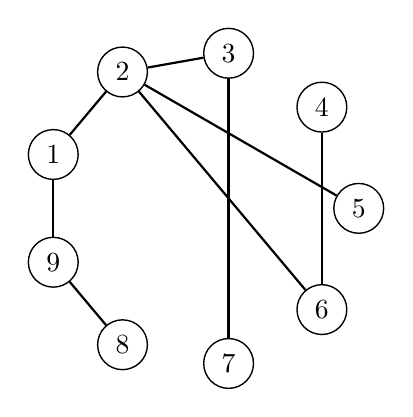
\begin{tikzpicture}
\GraphInit[vstyle=Normal]
\SetGraphUnit{2}
\Vertices{circle}{5,4,3,2,1,9,8,7,6}
\Edges(8,9,1,2,5)
\Edges(2,3,7)
\Edges(4,6)
\Edges(2,6)
\end{tikzpicture}
\end{minipage}
\qquad
\begin{minipage}{0.6\linewidth}
\begin{solutionbox}{1.7in}    \vspace{1em} \\
 
\end{solutionbox}
\end{minipage}

\question \textit{Kleinberg, Jon. Algorithm Design (p. 108, q. 5).} A binary tree is a rooted tree in which each node has at most two children. Show by induction that in any binary tree the number of nodes with two children is exactly one less than the number of leaves. 

\nopagebreak

\begin{solutionbox}{5in}    \vspace{1em}                                             

\end{solutionbox}


\pagebreak
\question \textit{Kleinberg, Jon. Algorithm Design (p. 108, q. 7).} Some friends of yours work on wireless networks, and they're currently studying the properties of a network of $n$ mobile devices. As the devices move around, they define a graph at any point in time as follows: 

{\leftskip=1cm\relax
 \rightskip=1cm\relax
 There is a node representing each of the $n$ devices, and there is an edge between device $i$ and device $j$ if the physical locations of $i$ and $j$ are no more than 500 meters apart. (If so, we say that $i$ and $j$ are “in range” of each other.)
 \par}

They'd like it to be the case that the network of devices is connected at all times, and so they've constrained the motion of the devices to satisfy the following property: at all times, each device $i$ is within 500 meters of at least $\frac{n}{2}$ of the other devices. (We'll assume $n$ is an even number.) What they'd like to know is: Does this property by itself guarantee that the network will remain connected? \\

Here’s a concrete way to formulate the question as a claim about graphs.\\

\textbf{Claim: Let $G$ be a graph on $n$ nodes, where $n$ is an even number. If every node of $G$ has degree at least $\frac{n}{2}$, then $G$ is connected.} \\

Decide whether you think the claim is true or false, and give a proof of either the claim or its negation. 

\begin{solutionbox}{4.5in} \vspace{1em}    

\end{solutionbox}

\pagebreak



\section*{Coding Question}
\question
Implement depth-first search in either C, C++, C\#, Java, or Python. Given an undirected graph with $n$ nodes and $m$ edges, your code should run in $O(n + m)$ time. Remember to submit a makefile along with your code, just as with week 1's coding question.\\

\textbf{Input:} the first line contains an integer $t$, indicating the number of instances that follows. For each instance, the first line contains an integer $n$, indicating the number of nodes in the graph. Each of the following $n$ lines contains several space-separated strings, where the first string $s$ represents the name of a node, and the following strings represent the names of nodes that are adjacent to node $s$. You can assume that the nodes are listed line-by-line in lexicographic order (0-9, then A-Z, then a-z), and the adjacent nodes of a node are listed in lexicographic order. For example, consider two consecutive lines of an instance:
\begin{verbatim}
0, F
B, C, a
\end{verbatim}
Note that 0 $<$ B and C $<$ a.\\

\textbf{Input constraints:}
\begin{itemize}
    \item $1 \leq t \leq 1000$
    \item $1 \leq n \leq 100$
    \item Strings only contain alphanumeric characters
    \item Strings are guaranteed to be the names of the nodes in the graph.
\end{itemize}

\textbf{Output:} for each instance, print the names of nodes visited in depth-first traversal of the graph, \emph{with ties between nodes visiting the first node in input order}. Start your traversal with the first node in input order. The names of nodes should be space-separated, and each line should be terminated by a newline.\\

\textbf{Sample:}
\begin{multicols}{2}
\textbf{Input:} 
\begin{verbatim}
2
3
A B
B A
C
9
1 2 9
2 1 6 5 3
4 6
6 2 4
5 2
3 2 7
7 3
8 9
9 1 8
\end{verbatim}
\columnbreak
\textbf{Output:} 
\begin{verbatim}
A B C
1 2 6 4 5 3 7 9 8
\end{verbatim}
\end{multicols}

The sample input has two instances. 
The first instance corresponds to the graph below on the left. 
The second instance corresponds to the graph below on the right.
\begin{center}
\begin{minipage}{0.3\linewidth}
    \begin{tikzpicture}
        \GraphInit[vstyle=Normal]
        \SetGraphUnit{2}
        \Vertices{circle}{A,B,C}
        \Edges(A,B)
    \end{tikzpicture}
\end{minipage}
\qquad\qquad
\begin{minipage}{0.3\linewidth}
    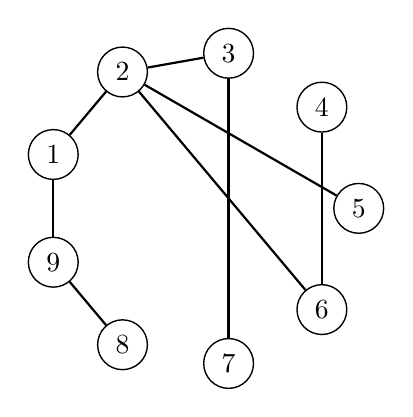
\begin{tikzpicture}
        \GraphInit[vstyle=Normal]
        \SetGraphUnit{2}
        \Vertices{circle}{5,4,3,2,1,9,8,7,6}
        \Edges(8,9,1,2,5)
        \Edges(2,3,7)
        \Edges(4,6)
        \Edges(2,6)
    \end{tikzpicture}
\end{minipage}

\hfill
\end{center}

\end{questions}

\end{document}